\documentclass[12pt]{article}
\usepackage[left=1cm, right=1cm, top=2cm,bottom=1.5cm]{geometry} 

\usepackage[parfill]{parskip}
\usepackage[utf8]{inputenc}
\usepackage[T2A]{fontenc}
\usepackage[russian]{babel}
\usepackage{enumitem}
\usepackage[normalem]{ulem}
\usepackage{amsfonts, amsmath, amsthm, amssymb, mathtools}
\usepackage{tabularx}
\usepackage{hhline}

\usepackage{accents}
\usepackage{fancyhdr}
\pagestyle{fancy}
\renewcommand{\headrulewidth}{1.5pt}
\renewcommand{\footrulewidth}{1pt}

\usepackage{graphicx}
\usepackage[figurename=Рис.]{caption}
\usepackage{subcaption}
\usepackage{float}

%%Наименование папки откуда забирать изображения
\graphicspath{ {./images/} }

%%Изменение формата для ввода доказательства
\renewcommand{\proofname}{$\square$  \nopunct}
\renewcommand\qedsymbol{$\blacksquare$}

%%Изменение отступа на таблицах
\addto\captionsrussian{%
	\renewcommand{\proofname}{$\square$ \nopunct}%
}
%% Римские цифры
\newcommand{\RN}[1]{%
	\textup{\uppercase\expandafter{\romannumeral#1}}%
}

%% Для удобства записи
\newcommand{\MR}{\mathbb{R}}
\newcommand{\MQ}{\mathbb{Q}}
\newcommand{\MN}{\mathbb{N}}
\newcommand{\MTB}{\mathbb{T}}
\newcommand{\MI}{\mathrm{I}}
\newcommand{\MJ}{\mathrm{J}}
\newcommand{\MH}{\mathrm{H}}
\newcommand{\MT}{\mathrm{T}}
\newcommand{\MU}{\mathcal{U}}
\newcommand{\MV}{\mathcal{V}}
\newcommand{\MW}{\mathcal{W}}
\newcommand{\VN}{\varnothing}
\newcommand{\VE}{\varepsilon}

\theoremstyle{definition}
\newtheorem{defn}{Опр:}
\newtheorem{rem}{Rm:}
\newtheorem{prop}{Утв.}
\newtheorem{exrc}{Упр.}
\newtheorem{lemma}{Лемма}
\newtheorem{theorem}{Теорема}
\newtheorem{corollary}{Следствие}

\newenvironment{cusdefn}[1]
{\renewcommand\thedefn{#1}\defn}
{\enddefn}

\DeclareRobustCommand{\divby}{%
	\mathrel{\text{\vbox{\baselineskip.65ex\lineskiplimit0pt\hbox{.}\hbox{.}\hbox{.}}}}%
}
%Короткий минус
\DeclareMathSymbol{\SMN}{\mathbin}{AMSa}{"39}
%Длинная шапка
\newcommand{\overbar}[1]{\mkern 1.5mu\overline{\mkern-1.5mu#1\mkern-1.5mu}\mkern 1.5mu}
%Функция знака
\DeclareMathOperator{\sgn}{sgn}

%Функция ранга
\DeclareMathOperator{\rk}{\text{rk}}

%Обозначение константы
\DeclareMathOperator{\const}{\text{const}}

%Интеграл в большом формате
\DeclareMathOperator{\dint}{\displaystyle\int}
\newcommand{\ddint}[2]{\displaystyle\int\limits_{#1}^{#2}}
\newcommand{\ssum}[1]{\displaystyle \sum\limits_{n=1}^{\infty}{#1}_n}

\newcommand{\smallerrel}[1]{\mathrel{\mathpalette\smallerrelaux{#1}}}
\newcommand{\smallerrelaux}[2]{\raisebox{.1ex}{\scalebox{.75}{$#1#2$}}}

\newcommand{\smallin}{\smallerrel{\in}}
\newcommand{\smallnotin}{\smallerrel{\notin}}

\newcommand*{\medcap}{\mathbin{\scalebox{1.25}{\ensuremath{\cap}}}}%
\newcommand*{\medcup}{\mathbin{\scalebox{1.25}{\ensuremath{\cup}}}}%

\makeatletter
\newcommand{\vast}{\bBigg@{3.5}}
\newcommand{\Vast}{\bBigg@{5}}
\makeatother

%Промежуточное значение для sup\inf, поскольку они имеют разную высоту
\newcommand{\newsup}{\mathop{\smash{\mathrm{sup}}}}
\newcommand{\newinf}{\mathop{\mathrm{inf}\vphantom{\mathrm{sup}}}}

%Скалярное произведение
\DeclarePairedDelimiterX{\inner}[2]{\langle}{\rangle}{#1, #2}

%Подпись символов снизу
\newcommand{\ubar}[1]{\underaccent{\bar}{#1}}

%% Шапка для букв сверху
\newcommand{\wte}[1]{\widetilde{#1}}

\begin{document}
\lhead{Математический анализ - \RN{3}}
\chead{Шапошников С.В.}
\rhead{Лекция - 2}
\section*{Ряды с неотрицательными слагаемыми}

Ряды с неотрицательными слагаемыми полезно сравнивать друг с другом.
\begin{corollary}
	Пусть, начиная с некоторого номера, выполнено: 
	$$
	\forall n, \, c_1 b_n \leq a_n \leq c_2 b_n
	$$
	где $c_1, c_2 >0$ - фиксированы $\Rightarrow$ ряды $\ssum{a}$ и $\ssum{b}$ сходятся и расходятся одновременно.
\end{corollary}
Мы рассмотрели наборы примеров, один из которых это геометрическая прогрессия. Докажем несколько простых наблюдений, которые по сути своей состоят в сравнении данного ряда с геометрической прогрессией.
\begin{prop}(\textbf{Признак Даламбера})
	Пусть $a_n > 0$, тогда:
	\begin{enumerate}[label ={(\arabic*)}]
		\item Если $\underset{n \to \infty}{\overline{\lim}} \dfrac{a_{n+1}}{a_n} = q < 1$, то ряд $\ssum{a}$ сходится;
		\item Если $\underset{n \to \infty}{\underline{\lim}} \dfrac{a_{n+1}}{a_n} = q > 1$, то ряд $\ssum{a}$ расходится;
		\item Если $q = 1$, то ничего сказать нельзя;
	\end{enumerate}	
\end{prop}
\begin{proof}
	Вспомним, что $\underset{n \to \infty}{\overline{\lim}}c_n = \lim\limits_{n \to \infty}\sup\limits_{k > n} c_k$ и $\underset{n \to \infty}{\underline{\lim}}c_n = \lim\limits_{n \to \infty} \inf\limits_{k > n} c_k$. Тогда:
	\begin{enumerate}[label ={(\arabic*)}]
		\item $\lim\limits_{n \to \infty} \left(\sup\limits_{k > n} \dfrac{a_{k+1}}{a_k}\right) = q < 1 \Rightarrow$ некая последовательность точных верхних граней сходится к некоторому числу $q < 1$. Тогда пусть $q < q_0 < 1$, получим:
		$$
			\exists \, n_0 \colon \forall n > n_0, \, \sup\limits_{k > n} \dfrac{a_{k+1}}{a_k} < q_0 < 1 \Rightarrow \forall k > n_0 + 1, \, \dfrac{a_{k+1}}{a_k} < q_0 < 1
		$$ 
		Поскольку точная верхняя грань меньше, чем $q_0$, то все такие элементы $\dfrac{a_{k+1}}{a_k}$ тем более меньше, чем $q_0$. Отбросим элементы $a_1, a_2, \dotsc, a_{n_0 + 1}$. Далее считаем что $\forall k, \, \dfrac{a_{k+1}}{a_k} < q_0 < 1$. Тогда:
		$$
			a_n = a_1{\cdot} \dfrac{a_2}{a_1}{\cdot}\dfrac{a_3}{a_2}{\cdot}\dotsc{\cdot}\dfrac{a_n}{a_{n-1}} \leq a_1{\cdot}q_0{\cdot}q_0{\cdot} \dotsc {\cdot} q_0 = a_1 {\cdot} q_0^{n-1}
		$$
		Ряд $\displaystyle \sum\limits_{n = 1}^{\infty}a_1q_0^{n-1}$ сходится $\Rightarrow$ ряд $\ssum{a}$ тоже сходится; 
		\item $\lim\limits_{n \to \infty} \left(\inf\limits_{k > n} \dfrac{a_{k+1}}{a_k}\right) = q > 1 \Rightarrow$ тогда выпишем формально:
		$$
			\exists \, n_0 \colon \forall n > n_0, \, \inf\limits_{k > n} \dfrac{a_{k+1}}{a_k} > 1 \Rightarrow \forall k > n_0 + 1, \, \dfrac{a_{k+1}}{a_k} > 1 \Rightarrow a_{k+1} > a_k \Rightarrow a_{k} \nrightarrow 0
		$$
		Последовательность положительных чисел не может возрастать и одновременно стремиться к нулю. И таким образом, необходимое условие сходимости не выполняется;
	\end{enumerate}
\end{proof}
\newpage
\begin{prop}(\textbf{Признак Коши})
	Пусть $a_n \geq 0$, тогда:
	\begin{enumerate}[label ={(\arabic*)}]
		\item Если $\underset{n \to \infty}{\overline{\lim}} \sqrt[n]{a_n} = q < 1$, то ряд $\ssum{a}$ сходится;
		\item Если $\underset{n \to \infty}{\overline{\lim}} \sqrt[n]{a_n} = q > 1$, то ряд $\ssum{a}$ расходится;
		\item Если $q = 1$, то ничего сказать нельзя;
	\end{enumerate}
\end{prop}
\begin{rem}
	При расходимости в качестве $q$ вполне допустима $+\infty$.
\end{rem}
\begin{rem}
	Всё доказательство сведется к неравенству $a_n \leq q^n$ для какого-то $q$. Но лучше писать $\sqrt[n]{a_n} \leq q$ потому что корень из $n$ асимптотически убивает любой множитель при $q^n$. Например, при $a_n \leq n q^n$ можно увидеть, что асимптоически ничего не меняется: $\sqrt[n]{a_n} \leq q {\cdot} \sqrt[n]{n}$, где $\sqrt[n]{n} \to 1$.
\end{rem}
\begin{proof}\hfill
		\begin{enumerate}[label ={(\arabic*)}]
		\item $\lim\limits_{n \to \infty} \left(\sup\limits_{k > n} \sqrt[k]{a_k}\right) = q < 1$. Тогда будет верно следующее:
		$$
			\exists \, q_0 < 1 \wedge n_0 \colon \forall n > n_0, \, \sup\limits_{k > n} \sqrt[k]{a_k} < q_0 < 1 \Rightarrow \forall k > n_0 + 1, \, \sqrt[k]{a_k} < q_0 < 1 \Rightarrow a_k < q_0^k
		$$
		Тем самым, начиная с некоторого номера члены ряда мажорируются чистой геометрической прогрессией $\Rightarrow$ ряд $\ssum{a}$ сходится; 
		
		\item Верхний предел это наибольший из частичных пределов, тогда: 
		$$
			\exists \, \{n_k\} \colon \sqrt[\leftroot{-2}\uproot{3}n_k]{a_{n_k}} \to q > 1
		$$ 
		В частности: 
		$$
			\exists \, K \colon \forall k > K, \, \sqrt[\leftroot{-2}\uproot{3}n_k]{a_{n_k}} > 1 \Rightarrow a_{n_k} > 1
		$$
		Это в точности означает, что $a_n \nrightarrow 0$
	\end{enumerate}
\end{proof}
\begin{rem}
	Между критериями есть взаимосвязь: признак Даламбера $\Rightarrow$ признак Коши. При этом есть ряды, которые по признаку Даламбера не исследуется, но исследуется по признаку Коши. Типичный пример:
	$$
		\ssum{a} = \dfrac{1}{2} + \dfrac{1}{3} + \dfrac{1}{4} + \dfrac{1}{9} + \dotsc + \dfrac{1}{2^n} + \dfrac{1}{3^n} + \dotsc
	$$
	Поскольку будут иметься такие члены $a_n$, что отношение $\dfrac{a_{n+1}}{a_n}$ при больших $n$ будет уходить в бесконечность и признак Даламбера не даст адекватного результата.
\end{rem}
\newpage
\section*{Бесконечные произведения}
Пусть $\{b_n\}$ - числовая последовательность.

\begin{defn}
	Выражение $\displaystyle \prod\limits_{n=1}^{\infty}b_n$ называется \uwave{бесконечным произведением}, где $b_n$ называются \uwave{множителями}.
\end{defn}
\begin{defn}
	Выражение $ \prod_N = \displaystyle \prod\limits_{n=1}^{N}b_n$ называется \uwave{частичным произведением}.
\end{defn}

\begin{defn}
	Если существует конечный, отличный от нуля, предел $\lim\limits_{N \to \infty}  \prod_N$, то говорят, что \uwave{произведение сходится} и равно этому пределу: $\lim\limits_{N \to \infty}  \prod_N \neq 0$.
\end{defn}
\begin{defn}
	Если $\lim\limits_{N \to \infty}  \prod_N = 0$, то говорят, что \uwave{произведение расходится к нулю}. В остальных случаях говорят, что  \uwave{произведение расходится}. 
\end{defn}

\begin{prop}(\textbf{Необходимое условие сходимости})
	Если $ \displaystyle\prod\limits_{n=1}^{\infty}b_n$ сходится, то $b_n \to 1$.
\end{prop}
\begin{proof}
	Поскольку бесконечное произведение сходится $\Rightarrow$ не к нулю $\Rightarrow$ среди $b_n$ нулей нет и частичные произведения точно отличны от нуля. Возьмем следующее отношение:
	$$
		b_n = \dfrac{ \prod_n\hfill}{ \prod_{n-1}} = \dfrac{\displaystyle \prod\limits_{k=1}^{n} b_k}{\displaystyle \prod\limits_{k=1}^{n-1} b_k} \xrightarrow{n \to \infty} \dfrac{\displaystyle \prod\limits_{k=1}^{\infty} b_k}{\displaystyle \prod\limits_{k=1}^{\infty} b_k} = 1
	$$
\end{proof}
\begin{rem}
	Поскольку $b_n$ в сходящихся бесконечных произведениях стремятся к единице, то начиная с некоторого номера они точно больше $0$. Точно также, как и в рядах можно отбрасывать конечное число множителей если они не нулевые, потому что делим фиксированные суммы на число или умножаем на фиксированное число.
\end{rem}
\begin{theorem}
	Пусть $b_n > 0$, тогда $\displaystyle \prod\limits_{n=1}^{\infty}b_n$ сходится $\Leftrightarrow \displaystyle\sum\limits_{n=1}^{\infty}\ln{b_n}$ сходится. В случае сходимости имеют место равенства:
	$$
		e^{ \sum\limits_{n = 1}^{\infty}\ln b_n} = \prod\limits_{n=1}^{\infty}b_n
	$$
	$$
		\ln\left(\prod\limits_{n=1}^{\infty}b_n\right) = \sum\limits_{n = 1}^{\infty}\ln b_n
	$$
\end{theorem}
\begin{proof}
	Функции $e^x, \, \ln x$ - непрерывные, верны формулы $e^{ \sum\limits_{n = 1}^{N}\ln b_n} = \displaystyle \prod\limits_{n = 1}^{N}b_n$ и $\ln\left(\displaystyle\prod\limits_{n=1}^{N}b_n\right) = \displaystyle \sum\limits_{n = 1}^{N }\ln b_n$. Здесь важно, что мы запретили произведению сходится к нулю. 
	
	$(\Rightarrow)$ Если $\displaystyle \prod\limits_{n = 1}^{\infty}b_n$ - сходится, то по определению $\lim\limits_{N\to \infty} \displaystyle \prod\limits_{n = 1}^{N}b_n = C > 0$. Так как $\ln x$ непрерывен на $(0, +\infty)$, то верно следующее $\ln\left(\prod\limits_{n=1}^{N}b_n\right) \xrightarrow[N \to \infty]{} \ln C$, но $\ln\left(\prod\limits_{n=1}^{N}b_n\right) = \displaystyle \sum\limits_{n = 1}^{N }\ln b_n \Rightarrow$ ряд из $\ln b_n$ - сходится.
	
	$(\Leftarrow)$ Если $\displaystyle \sum\limits_{n = 1}^{\infty}\ln b_n$ - сходится, то по определению $\lim\limits_{N\to \infty} \displaystyle \sum\limits_{n = 1}^{N}\ln b_n = C$. Так как $e^x$ непрерывна на $\MR$, то верно следующее $e^{ \sum\limits_{n = 1}^{N}\ln b_n} \xrightarrow[N \to \infty]{} e^C$, но $e^{ \sum\limits_{n = 1}^{N}\ln b_n} =\displaystyle \prod\limits_{n = 1}^{N}b_n \Rightarrow$ бесконечное произведение из $b_n$ - сходится.
\end{proof}

Мы знаем, что $b_n \to 1$, это можно записать как $b_n = 1 + \beta_n, \, \beta_n \to 0$. Предполагаем, что $b_n > 0$, но это вовсе не означает, что $\beta_n > 0$. Согласно предыдущей теореме, исследование сходимости бесконечного произведения свелось бы к исследованию ряда: 
$$
	\displaystyle \sum\limits_{n = 1}^{\infty}\ln(1 + \beta_n)
$$
Из прошлой лекции мы знаем, что знакопеременный ряд нельзя проверять асимптотическими методами по первому приближению. Нужен знакопостоянный ряд.
\begin{prop}
	Следующий ряд $\displaystyle \sum\limits_n \left| \ln(1 + \beta_n) \right|$ - сходится $\Leftrightarrow \displaystyle \sum\limits_n \left| \beta_n \right|$ - сходится. В частности, если сумма модулей $\displaystyle \sum\limits_n \left| \beta_n \right|$ - сходится, то и бесконечное произведение $\displaystyle \prod\limits_{n = 1}^{\infty}(1 + \beta_n)$ - сходится.
\end{prop}
\begin{proof}
	Мы знаем, что:
	$$
		\lim\limits_{x \to 0}\left| \dfrac{\ln(1+x)}{x} \right| =  1
	$$
	Пусть $\VE = \frac{1}{2}$, тогда:
	$$
		\exists \, \delta > 0 \colon \forall x \in (-\delta, \delta) \setminus \{0\}, \, -\dfrac{1}{2} \leq  \left| \dfrac{\ln(1+x)}{x} \right| -1 \leq \dfrac{1}{2} \Rightarrow \forall x \in (-\delta, \delta), \, \dfrac{1}{2} |x| \leq | \ln(1+ x)| \leq \dfrac{3}{2}|x|
	$$
	Далее рассматриваем только случай $\beta_n$ стремящегося к нулю (так получится для доказательства в обе стороны по необходимому условию сходимости).
	$$	
		\exists \, n_0 \colon \forall n > n_0, \, \dfrac{1}{2}|\beta_n| \leq |\ln(1+ \beta_n)| \leq \dfrac{3}{2}|\beta_n|
	$$
	Таким образом, слагаемые одного ряда оцениваются слагаемыми другого с константами $\Rightarrow$ по следствию сходимости рядов с неотрицательными слагаемыми оба ряда сходятся и расходятся одновременно $\Rightarrow$ требуемое - выполнено.
\end{proof}

\begin{rem}
	Заметим, что модуль убрать нельзя, иначе сыграют слагаемые более глубокого разложения логарифма (второго порядка).
\end{rem}

\begin{exrc}
	Доказать, что из сходимости рядов $\displaystyle \sum\limits_n \beta_n$ и $\displaystyle \sum\limits_n\beta_n^2$ следует сходимость ряда $\displaystyle \sum\limits_n \ln(1 + \beta_n)$. \textbf{Указание}: $\ln(1+ x) = x - \dfrac{x^2}{2} + o(x^2)$ .
\end{exrc}
\begin{proof}
	Воспользуемся разложением ряда Тейлора функции $\ln(1+x)$:
	$$
		\ln(1 + \beta_n) =\beta_n -  \dfrac{\beta_n^2}{2} + o(\beta_n^2) \Rightarrow \beta_n - \ln(1 + \beta_n) = \dfrac{\beta_n^2}{2} + o(\beta_n^2)
	$$
	Рассмотрим предел следующего отношения:
	$$
		\lim\limits_{n \to \infty}\dfrac{\left|\beta_n - \ln(1 + \beta_n)\right|}{\beta_n^2} = \lim\limits_{n \to \infty}\dfrac{\left|\dfrac{\beta_n^2}{2} + o(\beta_n^2)\right|}{\beta_n^2} = \lim\limits_{n \to \infty} \left|\dfrac{1}{2} + \dfrac{o(\beta_n^2)}{\beta_n^2} \right| = \dfrac{1}{2}
	$$
	Таким образом, по следствию из прошлой лекции ряды $\beta_n^2$ и $\left|\beta_n - \ln(1 + \beta_n)\right|$ сходятся одновременно. Первый ряд по условию сходится $\Rightarrow$ ряд $\beta_n - \ln(1 + \beta_n)$ сходится абсолютно $\Rightarrow$ сходится. Таким образом:
	$$
		\exists \, \lim\limits_{N \to \infty} \sum\limits_{n = 1}^{N}(\beta_n - \ln(1 + \beta_n)) = \lim\limits_{N \to \infty} \sum\limits_{n = 1}^{N}\beta_n  - \lim\limits_{N \to \infty} \sum\limits_{n = 1}^{N}\ln(1 + \beta_n)
	$$
	А поскольку ряд $\displaystyle \sum\limits_n \beta_n$ сходится, то существует предел частичной суммы $\Rightarrow$ существует предел частичной суммы второго слагаемого в правой части выше $\Rightarrow$ ряд $\displaystyle \sum\limits_n \ln(1 + \beta_n)$ также будет сходится.
\end{proof}

\begin{exrc}
	Привести пример, когда обратное утверждение не верно. То есть ряд $\displaystyle \sum\limits_n \ln(1 + \beta_n)$ сходится, но ряды $\displaystyle \sum\limits_n \beta_n$ и $\displaystyle \sum\limits_n\beta_n^2$ расходятся.
\end{exrc}
\begin{proof}
	Рассмотрим следующий ряд: $\forall n \in \MN, \, \beta_{2n -1} = \dfrac{1}{\sqrt{n}} + \dfrac{1}{n}, \, \beta_{2n} = -\dfrac{1}{\sqrt{n}}$.
	
	Ряд $\displaystyle \sum\limits_{n = 1}^{2N} \beta_n = \sum\limits_{n = 1}^{N} \dfrac{1}{n} \Rightarrow \displaystyle \sum\limits_{n = 1}^{\infty} \beta_n = \sum\limits_{n = 1}^{\infty} \dfrac{1}{n} \Rightarrow$ расходится. 
	
	Аналогично, $\beta_{2n-1}^2 + \beta_{2n}^2 = \dfrac{2}{n} + \dfrac{2}{n\sqrt{n}} + \dfrac{1}{n^2} \geq \dfrac{1}{n}, \, \forall n \in \MN$ и таким образом, ряд $\displaystyle \sum\limits_{n = 1}^{2N} \beta_n^2 \geq \sum\limits_{n = 1}^{N} \dfrac{1}{n} \Rightarrow$ по следствию из прошлой лекции, ряд $\displaystyle \sum\limits_{n = 1}^{\infty} \beta_n^2$ расходятся вместе с рядом $\sum\limits_{n = 1}^{\infty} \dfrac{1}{n}$.
	
	Рассмотрим $\displaystyle \prod\limits_n (1 + \beta_n)$, если этот ряд сходится, то $\displaystyle \sum\limits_n \ln(1 + \beta_n)$ также будет сходиться. Верно следующее: $\forall n \in \MN, \, (1 + \beta_{2n-1})(1 + \beta_{2n}) = 1 + \dfrac{1}{\sqrt{n}} + \dfrac{1}{n} - \dfrac{1}{\sqrt{n}} - \dfrac{1}{n} - \dfrac{1}{n\sqrt{n}} = 1 - \dfrac{1}{n\sqrt{n}}$, следовательно получим:
	$$
		\displaystyle \prod\limits_{n = 1}^{2N}(1 + \beta_n) = \prod\limits_{n = 1}^{N}\left(1 - \dfrac{1}{n\sqrt{n}}\right) = \prod\limits_{n = 1}^{N}\left(1 - \dfrac{1}{n^{\frac{3}{2}}}\right)
	$$
	Поскольку ряд $\displaystyle \sum\limits_{n = 1}^{\infty}\left|\dfrac{1}{n^{\frac{3}{2}}}\right|$ сходится, то сходится и правая часть уравнения выше, а значит и $\displaystyle \prod\limits_n (1 + \beta_n)$.
\end{proof}

\newpage
\section*{Разложение $\sin x$ в бесконечное произведение}
Пусть $P(x)$ - многочлен и $x_1, \dotsc, x_n$ - его корни. Тогда разложим многочлен на множители:
$$
	P(x) = A(x - x_1){\cdot} \dotsc {\cdot} (x - x_n)
$$
Если раскладывать по аналогии $\sin x$, то получим:
$$
	\sin x = A \prod\limits_n (x - \pi n)
$$
но такое произведение не является сходящимся. Преобразуем разложение многочлена:
$$
	P(x) = (-1)^nAx_1 {\cdot}\dotsc {\cdot}x_n {\cdot} \left(1 - \dfrac{x}{x_1}\right){\cdot}\dotsc{\cdot}\left(1 - \dfrac{x}{x_n}\right) = C{\cdot}\left(1 - \dfrac{x}{x_1}\right){\cdot}\dotsc{\cdot}\left(1 - \dfrac{x}{x_n}\right)
$$
Представим аналогичным способом разложение синуса. Учитывая что $n$ бегают по всем целым, соберем разность квадратов и получим следующее разложение:
$$
	\sin x = (x-0){\cdot} \prod\limits_{n = 1}^{\infty}\left(1 - \dfrac{x^2}{\pi^2 n^2}\right) = x \prod\limits_{n = 1}^{\infty}\left(1 - \dfrac{x^2}{\pi^2 n^2}\right)
$$
\begin{rem}
	Такое разложение возможно не только для функции $\sin{x}$, в комплексном анализе рассматриваются целые классы функции раскладывающиеся по нулям.
\end{rem}
\begin{theorem}(\textbf{Эйлера})
	$$
		\sin x = x \prod\limits_{n = 1}^{\infty}\left(1 - \dfrac{x^2}{\pi^2 n^2}\right)
	$$
\end{theorem}
\begin{rem}
	Выражение в правой части сходится при всех $x \neq \pi n$, а при $x = \pi n$ расходится к нулю. Поэтому можно считать, что равенство имеет место для всех $x \in \MR$.
\end{rem}
\begin{proof}
	Мы знаем из школы, что $\sin{(2N + 1)t} = \sin{t} {\cdot}P_N(\sin^2{t})$, где $P_N(x)$ - многочлен степени $N$.
	\begin{exrc}
		Доказать данное выражение по индукции, рассмотрев сумму: $\sin(2N + 3)t + \sin(2N - 1)t$.
	\end{exrc}
	\begin{proof}
		Воспользуемся формулой сложения синусов и косинуса двойного угла:
		$$
			\sin{(2N + 3)t} + \sin{(2N - 1)t} = 2\sin{(2N + 1)t}{\cdot}\cos{2t} = 2\sin{(2N + 1)t}{\cdot}(1 - 2 \sin^2{t})
		$$
		\uline{База}: $\sin{3t} = \sin{t}{\cdot}P_1(\sin^2{t})$, разложим $\sin{3t}$:
		$$
			\sin{3t} = \sin{2t +t} = \sin{2t}{\cdot}\cos{t} + \cos{2t}{\cdot}\sin{t} = (2\sin{t}{\cdot}\cos{t}){\cdot}\cos{t} + (1 - 2\sin^2{t}){\cdot}\sin{t} = 
		$$
		$$
			= 2\sin{t}{\cdot}(1 - \sin^2{t}) + (1 - 2\sin^2{t}){\cdot}\sin{t} = 3\sin{t} - 4\sin^3{t} = \sin{t}{\cdot}(3 - 4\sin^2{t}) = \sin{t}{\cdot}P_1(\sin^2{t})
		$$
		Или, используя формулу выше при $N = 0$, получим аналогичное:
		$$
			\sin{3t} + \sin{(-t)} = 2\sin{t}{\cdot}(1- 2\sin^2{t}) \Rightarrow \sin{3t} = 3\sin{t} - 4\sin^3{t}
		$$
		\uline{Шаг}: пусть выражение верно для $N \colon \sin{(2N + 1)t} = \sin{t} {\cdot}P_N(\sin^2{t})$, рассмотрим случай $N+1$:
		$$
			(2(N+1) + 1)t = (2N + 3)t \Rightarrow \sin{(2N + 3)t} = 2\sin{(2N + 1)t}{\cdot}(1 - 2 \sin^2{t}) - \sin{(2N - 1)t}
		$$
		По индукции верно: $\sin{(2N - 1)t} = \sin{t}{\cdot}P_{N-1}(\sin^2{t})$ и $\sin{(2N + 1)t} = \sin{t}{\cdot}P_{N}(\sin^2{t})$, тогда получим:
		$$
			\sin{(2N + 3)t} = 2\sin{t}{\cdot}P_{N}(\sin^2{t}){\cdot}(1 - 2 \sin^2{t}) - \sin{t}{\cdot}P_{N-1}(\sin^2{t}) = \sin{t}{\cdot}(P_{N+1}(\sin^2{t}) - P_{N-1}(\sin^2{t}))
		$$
		где последнее равенство верно, поскольку умножение многочлена степени $N$ на многочлен степени $1$ дает новый многочлен степени $N+1$, тогда:
		$$
			\sin{(2N + 3)t}	= \sin{t}{\cdot}(P_{N+1}(\sin^2{t})) 
		$$
		где последнее верно в силу того, что степени многочленов различны и максимальная степень равна $N+1$. Таким образом, получили требуемое.
	\end{proof}
	Перепишем исходное выражение в следующем виде:
	$$
		\dfrac{\sin{(2N + 1)t}}{\sin{t}} = P_N(\sin^2{t})
	$$
	Корни этого многочлена можно найти из равенства нулю левой части: 
	$$
		(2N + 1)t = \pi n \Rightarrow t = \dfrac{\pi n}{2N + 1} \Rightarrow \sin^2 \left(\dfrac{\pi n}{2N + 1}\right)
	$$
	
	Теперь, когда $n$ будет пробегать $1,2, \dotsc, N$ наберём как раз $N$ различных корней, а потом он пойдет на повтор (поскольку от $0$ до $\dfrac{\pi}{2}$ квадрат синуса возрастает). Следовательно, можно будет многочлен разложить на множители:
	$$
		\dfrac{\sin{(2N + 1)t}}{\sin{t}} = P_N(\sin^2 t) = C_N{\cdot}\prod\limits_{n = 1}^N\left(1 - \dfrac{\sin^2 t}{\sin^2 \frac{\pi n}{2N + 1}}\right)
	$$
	Как найти константу? Пусть $t \to 0$ тогда слева будет стремление к $2N + 1$ по замечательному пределу, а справа к $C_N$. Следовательно, получим что $C_N = (2N + 1)$. 
	
	Возьмем $t = \dfrac{x}{2N+1}$, тогда получим:
	$$
		\sin x = (2N + 1){\cdot}\sin{ \dfrac{x}{2N+1}}{\cdot} \prod\limits_{n = 1}^N \left(1 - \dfrac{\sin^2 \tfrac{x}{2N + 1}}{\sin^2 \tfrac{\pi n}{2N +1}}\right)
	$$
	\textbf{Эвристически}: Устремляем $N \to \infty$ и пользуемся замечательными пределами $\Rightarrow$ получим требуемое. Но проблема в том, что нельзя устремлять $N$ и в множителях, и в их количестве. Поэтому этот предельный переход требует обоснования.
	
	\textbf{(Продолжение доказательства из лекции 3)}: 
	Разделим полученный многочлен на главную и хвостовую части:
	$$
		\sin{x} = \left[(2N + 1){\cdot}\sin{ \dfrac{x}{2N+1}}{\cdot} \prod\limits_{n = 1}^J \left(1 - \dfrac{\sin^2 \tfrac{x}{2N + 1}}{\sin^2 \tfrac{\pi n}{2N +1}}\right)
		\right]
		{\cdot}
		\prod\limits_{n = J + 1}^N \left(1 - \dfrac{\sin^2 \tfrac{x}{2N + 1}}{\sin^2 \tfrac{\pi n}{2N +1}}\right)
	$$
	Поскольку тождество верно $\forall N$, устремим $N \to \infty$, тогда:
	$$
		\lim\limits_{N \to \infty} (2N + 1){\cdot}\sin{ \dfrac{x}{2N+1}} = x, \, \lim\limits_{N \to \infty}\prod\limits_{n = 1}^J \left(1 - \dfrac{\sin^2 \tfrac{x}{2N + 1}}{\sin^2 \tfrac{\pi n}{2N +1}}\right) = \prod\limits_{n = 1}^J\left(1 - \dfrac{x^2}{\pi^2 n^2}\right)
	$$
	У первой части тождества есть конечный предел, значит есть конечный предел и у второй части тождества, обозначием его $R_J$:
	$$
		\lim\limits_{N \to \infty} \prod\limits_{n = J + 1}^N \left(1 - \dfrac{\sin^2 \tfrac{x}{2N + 1}}{\sin^2 \tfrac{\pi n}{2N +1}}\right) = R_J
	$$
	Нам необходимо как-то этот предел оценить, поскольку мы хотим получить бесконечное произведение. Если покажем, что $\lim\limits_{J \to \infty} R_J = 1$, то всё будет доказано. Мы получили, что $\forall J$ верно:
	$$
		\sin{x} = x{\cdot}\prod\limits_{n = 1}^J\left(1 - \dfrac{x^2}{\pi^2 n^2}\right){\cdot}R_J
	$$
	Очевидна оценка сверху (поскольку идет перемножение членов, меньше единицы):
	$$
		\prod\limits_{n = J + 1}^N \left(1 - \dfrac{\sin^2 \tfrac{x}{2N + 1}}{\sin^2 \tfrac{\pi n}{2N +1}}\right) \leq 1
	$$
	Найдем оценку снизу. Вспоминая, что если угол $x$ был в интервале $\left(0, \tfrac{\pi}{2}\right)$, то $\sin{x} \leq x$. И поскольку $\sin{x}$ на этом интервале это выпуклая функция, то она больше секущей на нём $\Rightarrow \sin{x} \geq \tfrac{2}{\pi}x$.
	\begin{figure}[H]
		\centering
		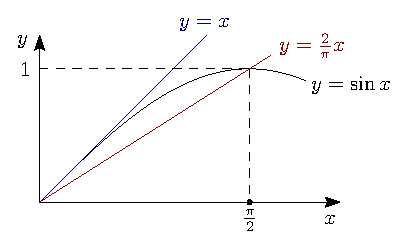
\includegraphics[width=0.4\textwidth]{MA3_2_1.eps}
		\label{2_1}
		\caption{Оценка функции $\sin{x}$ на интервале $\left(0, \tfrac{\pi}{2}\right)$.}
		\label{fig:Оценка синуса}
	\end{figure}	
	Таким образом:
	$$
		\forall x \in \left(0, \tfrac{\pi}{2}\right), \, \dfrac{2}{\pi}x \leq \sin{x} \leq x 
	$$
	Возьмем $J$ достаточно большим так, чтобы $\forall N > J, \, \dfrac{|x|}{2N + 1} \in \left(0, \tfrac{\pi}{2}\right)$, тогда:
	$$
		\dfrac{\sin^2 \tfrac{x}{2N + 1}}{\sin^2 \tfrac{\pi n}{2N +1}} \leq \dfrac{\tfrac{x^2}{(2N+1)^2}}{\tfrac{4\pi^2 n^2}{\pi^2(2N+1)^2}} = \dfrac{x^2}{4n^2}	
	$$
	Следовательно, получили оценку снизу для достаточно больших $J$:
	$$
		\prod\limits_{n = J + 1}^N \left(1 - \dfrac{x^2}{4n^2}\right) \leq
		\prod\limits_{n = J + 1}^N \left(1 - \dfrac{\sin^2 \tfrac{x}{2N + 1}}{\sin^2 \tfrac{\pi n}{2N +1}}\right) \leq 1
	$$
	Перейдем к пределу по $N$, поскольку $\displaystyle \sum\limits_n \left|\dfrac{x^2}{4n^2}\right|$ сходится, то произведение $\displaystyle \prod\limits_{n} \left(1 - \dfrac{x^2}{4n^2}\right)$ сходится и мы получим следующие неравенства:
	$$
		\prod\limits_{n = J + 1}^{\infty} \left(1 - \dfrac{x^2}{4n^2}\right) \leq R_J \leq 1
	$$
	Устремим $J \to \infty$, тогда получим:
	$$
		\lim\limits_{J \to \infty}\prod\limits_{n = J + 1}^{\infty} \left(1 - \dfrac{x^2}{4n^2}\right) =
		\lim\limits_{J \to \infty}\dfrac{\prod\limits_{n = 1}^{\infty} \left(1 - \dfrac{x^2}{4n^2}\right)}{\prod\limits_{n = 1}^{J} \left(1 - \dfrac{x^2}{4n^2}\right)} = 1 \Rightarrow \lim\limits_{J \to \infty} R_J = 1
	$$
	Следовательно, используя сходимость $\displaystyle \sum\limits_n \left|\dfrac{x^2}{4n^2}\right|$, получим требуемое:
	$$
		\sin{x} = \lim\limits_{J \to \infty} \left(x{\cdot}\prod\limits_{n = 1}^J\left(1 - \dfrac{x^2}{\pi^2 n^2}\right){\cdot}R_J \right) = x{\cdot}\prod\limits_{n = 1}^{\infty}\left(1 - \dfrac{x^2}{\pi^2 n^2}\right){\cdot}1 = x{\cdot}\prod\limits_{n = 1}^{\infty}\left(1 - \dfrac{x^2}{\pi^2 n^2}\right)
	$$
\end{proof}


\end{document}